\chapter{Colisiones Moleculares: tratamiento cl\'{a}sico}
\label{C:colis-molec}


\section{Potenciales}
\label{S:potenciales}

Para el potencial intramolecular consideramos un t\'{e}rmino el\'{a}stico arm\'{o}nico de cada fl\'{u}or con el \'{a}tomo central y t\'{e}rminos arm\'{o}nicos de ``bending'' entre los fl\'{u}or que dependen de su \'{a}ngulo
\begin{equation}\label{Q:pot-intra-energy}
  U = \sum_{\ell=1}^{6} K_{R} (r_{\ell X} - r_{0})^{2} + \sum_{\ell=1}^{6} \sum_{\ell'=\ell + 1}^{6} K_{\theta} (\theta_{\ell \ell'} - \theta_{0})
\end{equation}
%
donde $\theta_{0}=90^{\circ}$  en este caso.
  \begin{figure}[htbp]
\begin{minipage}{0.45\textwidth}
    % \centering \resizebox{.8\linewidth}{!}{\begin{tikzpicture}
\GraphInit[vstyle = Shade]
\Huge
\tikzset{
  % LabelStyle/.style = {font = \bfseries},
  VertexStyle/.append style = { inner sep=5pt, minimum size=40pt ,
                                font = \bfseries},
  EdgeStyle/.append style = {->},
}

  \SetGraphUnit{5}
  \begin{scope}
    \tikzset{VertexStyle/.append style = {%
        shape= circle, shading= ball, ball color= red!80!white,%
        minimum size = 50pt,draw} } 
    \Vertex[L=X]{X}
  \end{scope}


  \EA[L=$\bf{F}_{\ell}$](X){F}
  \WE[NoLabel](X){C}
  \NO[NoLabel](X){D}
  \SO[NoLabel](X){E}

  \Vertex[x=2, y=2, NoLabel]{A}
  \Vertex[x=-2, y=-2, NoLabel]{B}
  
  \begin{scope}
    \tikzset{VertexStyle/.append style = {%
      shape= circle,shading= ball,ball color= green!80!white,%
      minimum size = 50pt,draw}
    }
    \Vertex[x=10, y=6]{P}
  \end{scope}

  \Edge[label = $\bf{r}_{\ell X}$](X)(F)
  \Edge[label = $\bf{r}_{\ell}$](F)(P)
  \Edge[label = $\bf{r}$](X)(P)
  

  \tikzset{EdgeStyle/.append style = {->, dashed}}

  \draw [->,very thick, dashed] (5.8,0) -- (9.5,0);
  \draw [->, very thick] (6.8,0) arc [start angle=0, end angle=80, radius=1.1];
  \node at (7.,1) {$\theta_{\ell}$};

  \draw [<->, very thick] (0.,-1.2) arc [start angle=-90, end angle=0, radius=1.2];
  \node at (1,-1.5) {$\theta_{\ell \ell'}$};

  \Edge(X)(C)
  \Edge(X)(D)
  \Edge(X)(E)
  \Edge(X)(A)
  \Edge(X)(B)

\end{tikzpicture}


}
    \centering 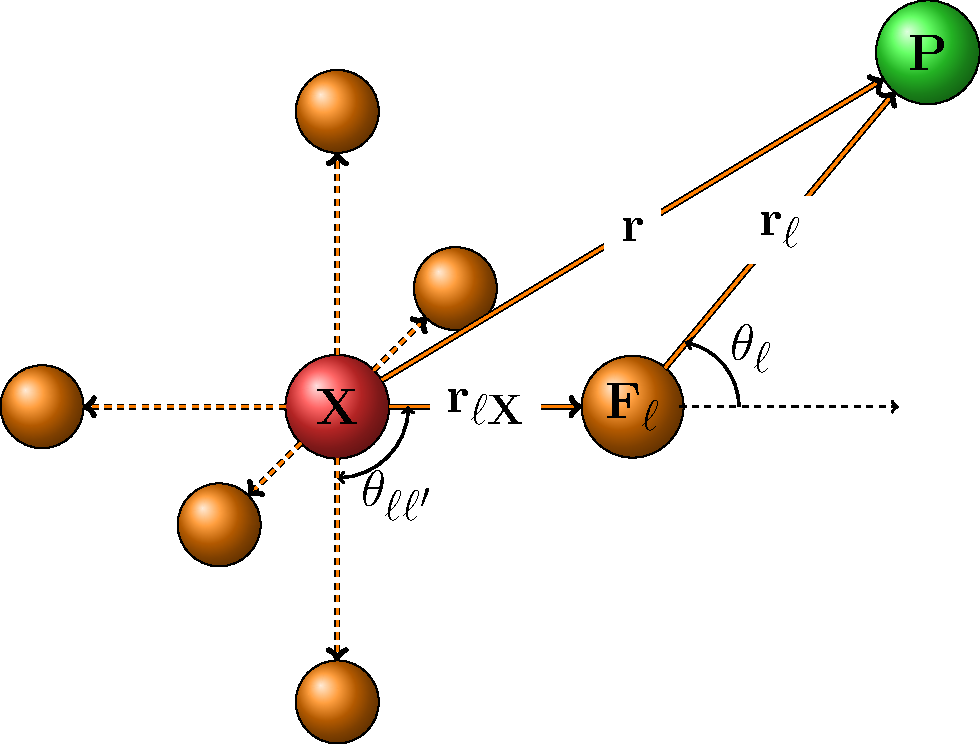
\includegraphics[width=.8\linewidth]{figures/coordenadas}
    \caption{Coordenadas utilizadas}
\end{minipage}\hfill
\begin{minipage}{0.5\textwidth}
  \begin{subequations}
    \begin{align}
      &\vect{r}=  \vect{r}_{\ce{P}} - \vect{r}_{X} , \\
      &\vect{r}_{\ell}=  \vect{r}_{\ce{P}} - \vect{r}_{\ce{F_{\ell}}} , \\
      &\vect{r}_{\ell X}= \vect{r}_{F_{\ell}} - \vect{r}_{X} ,
    \end{align}
  \end{subequations}
  \begin{itemize}
  \item $\theta_{\ell}$ es el \'{a}ngulo entre $\vect{r}_{\ell}$ y $\vect{r}_{\ell X}$,
  \item $\theta_{\ell \ell'}$ es el \'{a}ngulo entre $\vect{r}_{\ell}$ y $\vect{r}_{\ell'}$.
  \end{itemize}
\end{minipage}
\end{figure}

En el caso de colisiones de mol\'{e}culas de hexafluoruro de azufre (\ce{XF6}=\ce{SF6}) con un proyectil at\'{o}mico (en este caso $P=\ce{Ar}$) utilizamos para los potenciales intermoleculares las expresiones funcionales del grupo de Le Roy \autocite{Eichena1988TJCPp2898} y colaboradores (ver informe de Javier)
\begin{subequations}
  \begin{align} \label{Q:pot-inter-energy-1}
    U_{\ce{Ar-S}} &= - \sum_{n=3}^{5} \left[ 1 - \rme^{-br} \sum_{k=0}^{2n}\frac{(br)^{k}}{k!}\right] \frac{C_{2n}}{r^{2n}} \,,    \\
 \label{Q:pot-inter-energy-2}   U_{\ce{Ar-F_{\ell}}} &= A \Big[1 + p\, P_{2}(\cos \theta_{\ell})\Big]\, \rme^{-b r_{\ell}} - \sum_{n=3}^{5} \left[ 1 - \rme^{-br_{\ell}} \sum_{k=0}^{2n}\frac{(br_{\ell})^{k}}{k!}\right] \frac{C_{2n}}{r_{\ell}^{2n}}\,,
  \end{align}
\end{subequations}
$P_{2}(x)= 3 x^{2}/2 -1/2$ es el polinomio de Legendre de segundo orden.


\section{Fuerzas}
\label{S:calculo-fuerzas}
Las fuerzas se obtienen de las expresiones para la energ\'{\i}a potencial. Usaremos la aproximaci\'{o}n de que el potencial se puede escribir como una suma sobre potenciales de interacci\'{o}n de a pares entre \'{a}tomos. 

\subsection{Fuerzas intramoleculares}
Las fuerzas intra-moleculares se obtienen derivando la energ\'{\i}a (\ref{Q:pot-inter-energy-1}) y (\ref{Q:pot-inter-energy-2}) respecto a la coordenada respectiva:
%
\begin{subequations}
  \begin{align}\label{Q:F-sobre-X}
    &  \vect{F}^{\text{(i)}}_{X} = \sum_{\ell=1}^{6}\vect{F}^{\text{(i)}}_{X\ell} & \vect{F}^{\text{(i)}}_{X\ell} &=  2 K_{R} \, (r_{\ell X}- r_{0})\, \vers{r}_{\ell X}  \\
    & &  \vect{F}^{\text{(i)}}_{X\ell,i} &= 2 K_{R} \, \left( 1-\frac{r_{0}}{r_{\ell X}} \right) r_{\ell X,i}  \nonumber\\
    \label{Q:F-Sobre-Fl}
    &\vect{F}^{\text{(i)}}_{\ell} =   \vect{F}^{\text{(i)}}_{\ell X} + \sum_{\ell' \ne \ell} \vect{F}^{\text{(i)}}_{\ell \ell'} & \\
    &  & \vect{F}^{\text{(i)}}_{\ell X} &= -  \vect{F}^{\text{(i)}}_{X\ell} \nonumber \\
    & & \vect{F}^{\text{(i)}}_{\ell \ell'} &= -\frac{2 K_{\theta}}{r_{\ell X}} \frac{\theta_{\ell\ell'}-\theta_{0}}{\sin \theta_{\ell\ell'}} \Big[ \vers{r}_{\ell' X} - \cos{(\theta_{\ell\ell'})} \vers{r}_{\ell X} \Big] \nonumber
  \end{align}
\end{subequations}

\subsection{Fuerzas intermoleculares}

Como se muestra en el ap\'{e}ndice \ref{S:calculo-explicit-fuerzas} las fuerzas debidas a la presencia del proyectil est\'{a}n dadas por (\ref{Q:pot-inter-fuerzas}) y (\ref{Q:pot-inter-fuerza-S})

\begin{subequations}
  \begin{align}
    \label{Q:fuerzas-intermolec-resumen}
    \vect{F}^{\text{(e)}}_{\ell} =& - 3 A p \cos \theta_{\ell}\, \rme^{-b r_{\ell}} \vect{\Lambda} - A b \Big[1 + p\, P_{2}(\cos \theta_{\ell})\Big]\,\rme^{-b r_{\ell}} \vers{r_{\ell}} \nonumber \\
                                  &- \vers{r}_{\ell}\, \sum_{n=3}^{5} \frac{2 n\, C_{2n}}{r_{\ell}^{2n+1}} \,\left[ 1 - \frac{\rme^{-br_{\ell}}}{r_{\ell}} \left( \sum_{k=0}^{2n}\frac{(br_{\ell})^{k}}{k!} + \frac{(br_{\ell})^{2n+1}}{(2n)(2n)!} \right) \right] \\
    \vect{F}^{\text{(e)}}_{X} =&  3 A p \sum_{\ell=1}^{6} \cos \theta_{\ell}\, \rme^{-b r_{\ell}} \, \vect{\lambda} \\
    \vect{F}^{\text{(e)}}_{P} =& - \Bigl[ \vect{F}^{\text{(e)}}_{X} + \sum_{\ell} \vect{F}^{\text{(e)}}_{\ell}  \Bigr]
                                 \intertext{con}
                                  & \vect{\Lambda} = \left( \frac{1}{r_{\ell}} + \cos \theta_{\ell}\frac{1}{r_{\ell X}} \right) \vers{r}_{\ell X} - \left( \frac{1}{r_{\ell X}} + \cos \theta_{\ell}\frac{1}{r_{\ell}} \right) \vers{r}_{\ell} \\
                                  & \vect{\lambda}= \frac{1}{r_{\ell X}} \bigl( \vers{r}_{\ell} - \cos \theta_{\ell}\vers{r}_{\ell X} \bigr)
  \end{align}
\end{subequations}

\section{C\'{a}lculo del Jacobiano}
\label{S:calc-jacob}

El jacobiano del sistema de ecuaciones diferenciales para $N$ part\'{\i}culas interactuantes es una matriz de $6N \times 6N$, y tiene la forma
\begin{equation}
  \label{Q:Jacob-ec-dif}
  J =
  \begin{pmatrix}
    0 & A \\
    B & 0 \\
  \end{pmatrix}
\end{equation}
donde, en nuestro caso para \ce{XF6} con un proyectil $P=\ce{Ar}$, $N=8$, y la matriz $A$ est\'{a} formada por 8 bloques de $3 \times 3$, proporcionales a la identidad
\begin{align}
  \label{Q:Jacob-ec-dif-A}
  A &=
\begin{pmatrix}
  A_{X} & 0 & \cdots &  \cdots & 0 \\
  0 & A_{\ce{F1}}& 0 & \cdots & 0 \\
  \vdots  & \vdots  & \ddots &  & \vdots  \\
  0 &  0 &\cdots &  A_{\ce{F6}} & 0 \\
  0 & 0 & \cdots & 0 & P
\end{pmatrix}    &A_{j} = \frac{1}{M_{j}} \oper{I}^{(3\times 3)}
\end{align}

La matriz $B$ es de $(24\times 24)$ y contiene las derivadas de las fuerzas.
%
\begin{subequations}
  \begin{align}
    \label{Q:Jacob-eq-dif-B}
&   B =
\begin{pmatrix}
  BXX & BXF & BXP \\
  BFX & BFF & BFP \\
  BPX & BPF & BPP 
\end{pmatrix}   \\ \label{Q:Jacob-eq-dif-BXX}
    & BXX  & (BXX)_{i,j} = \frac{\partial F_{X,i}}{\partial r_{X,j}}  \\
\label{Q:Jacob-eq-dif-BXF}    &BXF =  \begin{pmatrix}   BXF_{1} & BXF_{2} & \cdots & BXF_{6}   \end{pmatrix}
    & (BXF_{\ell})_{i,j}=  \frac{\partial F_{X,i}}{\partial r_{\ell,j}}\\
\label{Q:Jacob-eq-dif-BFX}    &BFX =  \begin{pmatrix}   BF_{1}X \\ BF_{2}X \\ \cdots \\ BF_{6}X   \end{pmatrix}
    & (BF_{\ell}X)_{i,j}=  \frac{\partial F_{\ell,i}}{\partial r_{X,j}} \\ 
\label{Q:Jacob-eq-dif-BFF}    &BFF =  \begin{pmatrix}
  B11 & B12 & \cdots & B16 \\
  B21 & B22 & \cdots & B26 \\
  \vdots  & \vdots  & \ddots & \vdots  \\
  B61 & B62 & \cdots & B66 
 \end{pmatrix} & (B\ell\ell')_{i,j}=  \frac{\partial F_{\ell,i}}{\partial r_{\ell',j}}
  \end{align}
\end{subequations}
Usaremos la notaci\'{o}n $r_{X,i}$ para la componente $i=1,2,3$ (o sea $x,y,z$) del vector posici\'{o}n de la mol\'{e}cula $X$, e id\'{e}nticamente usaremos $r_{\ell, i}$ para la componente $i$ del vector posici\'{o}n del fl\'{u}or n\'{u}mero $\ell$. Similar notaci\'{o}n usamos para las componentes de la fuerza: $F_{X,i}$ es la componente $i$ de la fuerza total ejercida sobre el \'{a}tomo $X$.
Cada submatriz es de tama\~{n}o $3 \times 3$, donde $i,j= 1,2,3$  y $\ell,\ell'=1, \dots, 6$.

Las submatrices ($3 \times 3$) relacionadas con el proyectil tienen la forma 
\begin{align}
 & (BXP)_{i,j} =  \frac{\partial F_{X,i}}{\partial r_{P,j}} &
 & (BPX)_{i,j} =  \frac{\partial F_{P,i}}{\partial r_{X,j}} &  (BPP)_{i,j}=\frac{\partial F_{P,i}}{\partial r_{P,j}} \nonumber \\
\\
 & (BPF_{\ell})_{i,j}=  \frac{\partial F_{P,i}}{\partial r_{\ell,j}} &
 & (BF_{\ell}P)_{i,j}=  \frac{\partial F_{\ell,i}}{\partial r_{P,j}} & \forall \ell= 1, \dots, 6 \nonumber
\end{align}




\subsection{Relaciones entre los elementos de matriz}
\label{S:relaciones-elementos}


\subsubsection{Relaciones entre $BFX$, $BXF$ y $BXX$}
Para calcular $BFX$ consideramos como depende la fuerza sobre el \'{a}tomo \ce{X}  de la posici\'{o}n del fl\'{u}or $\ell$. 
Usamos que $\vect{r}_{\ell X} = \vect{r}_{\ell} - \vect{r}_{X}$
\begin{equation}
  \label{Q:BXF-1}
  (BXF_{\ell})_{ij} = \frac{\partial F_{X,i}}{\partial r_{\ell,j}} = \frac{\partial F_{X,i}}{\partial r_{\ell X,j}} \overbrace{\frac{\partial r_{\ell X,j}}{\partial r_{\ell,j}}}^{1} = \sum_{\ell'=1}^{6} \frac{\partial F_{X\ell',i}}{\partial r_{\ell X,j}} = \frac{\partial F_{X\ell,i}}{\partial r_{\ell X,j}}
\end{equation}

Para calcular el t\'{e}rmino $BF_{\ell}X$ debemos tener como var\'{\i}a la fuerza sobre el fl\'{u}or $\ell$ debido a movimientos de la posici\'{o}n del \'{a}tomo \ce{X}. En ese c\'{a}lculo debemos tener en cuenta que el \'{a}ngulo $\theta_{\ell \ell'} $ depende de la posici\'{o}n de \ce{X}.
Veamos si podemos pensarlo en forma diferente
\begin{equation}
  \label{Q:BFX-1}
  (BF_{\ell}X)_{ij} = \frac{\partial F_{\ell,i}}{\partial r_{X,j}} = \frac{\partial}{\partial r_{X,j}} \left(- \frac{\partial V}{\partial r_{\ell,i}}  \right) =
 \frac{\partial}{\partial r_{\ell,i}} \left(- \frac{\partial V}{\partial r_{X,j}}  \right) =  \frac{\partial F_{X,j}}{\partial r_{\ell,i}} = (BXF_{\ell})_{ji}
\end{equation}
por lo que tendremos $BFX=(BXF)^{t}$.

Para calcular $BXX$ consideramos el cambio en la fuerza sobre \ce{X} cuando var\'{\i}a su posici\'{o}n
\begin{equation}
  \label{Q:BXX-1}
  (BXX)_{ij} = \frac{\partial F_{X,i}}{\partial r_{X,j}} = \frac{\partial F_{X,i}}{\partial r_{\ell X,j}} \overbrace{\frac{\partial r_{\ell X,j}}{\partial r_{X,j}}}^{-1} = - \sum_{\ell=1}^{6} \frac{\partial F_{X\ell,i}}{\partial r_{\ell X,j}} = -\sum_{\ell=1}^{6} (BXF_{\ell})_{ij}
\end{equation}

\subsubsection{Relaciones entre $BFP$, $BPF$ y $BPP$}

Id\'{e}nticamente a la derivaci\'{o}n de las relaciones anteriores obtenemos
\begin{subequations}
  \begin{align}
    BPX &= (BXP)^{t}\\
    BPF_{\ell} &= (BF_{\ell}P)^{t} \\
    BPP &= - \sum_{\ell=1}^{6} {BF_{\ell}P} - BXP
  \end{align}
\end{subequations}

\subsubsection{Relaciones de submatrices en $BFF$}

En general, de (\ref{Q:Jacob-eq-dif-BFF}) podemos ver que:
\begin{equation}
  \label{Q:BFF-1}
  (B\ell\ell')_{ij} =  \frac{\partial F_{\ell,i}}{\partial r_{\ell',j}} = \frac{\partial}{\partial r_{\ell,j}} \left(- \frac{\partial V}{\partial r_{\ell',i}}  \right) =
 \frac{\partial}{\partial r_{\ell',i}} \left(- \frac{\partial V}{\partial r_{\ell,j}}  \right) =  \frac{\partial F_{\ell',j}}{\partial r_{\ell,i}} = (B\ell'\ell)_{ji} \,,
\end{equation}
% 
por lo que $B\ell\ell' = (B\ell'\ell)^{t}$.

Entonces, para $\ell = \ell'$ (matrices en la diagonal) $B\ell\ell = (B\ell\ell)^{t}$, y adem\'{a}s tendremos:
%
\begin{align*}
  (B\ell\ell)_{ij} =  \frac{\partial F_{\ell,i}}{\partial r_{\ell,j}} =  \frac{\partial }{\partial r_{\ell,j}} \left( {F}_{\ell X,i} + \sum_{\ell' \ne \ell} {F}_{\ell \ell',i} \right)
\intertext{donde}
   \frac{\partial F_{\ell X,i}}{\partial r_{\ell,j}} = - \frac{\partial F_{X \ell,i}}{\partial r_{\ell,j}} = - \frac{\partial F_{X \ell,i}}{\partial r_{\ell X,j}} \overbrace{\left( \frac{\partial r_{\ell X,j}}{\partial r_{\ell,j}} \right) }^{1} = - (BXF_{\ell})_{ij}
\intertext{y}
   \sum_{\ell' \ne \ell} \frac{\partial F_{\ell \ell',i}}{\partial r_{\ell,j}} = -  \sum_{\ell' \ne \ell} \frac{\partial F_{\ell' \ell,i}}{\partial r_{\ell,j}} = - \sum_{\ell' \ne \ell} (B\ell'\ell)_{ij}
\end{align*}
Por lo que
\begin{equation}
  \label{Q:BFF-diag-1}
  (B\ell\ell)_{ij} = (B\ell\ell)_{ji} = - (BXF_{\ell})_{ij} - \sum_{\ell' \ne \ell}(B\ell'\ell)_{ij}
\end{equation}

\subsection{C\'{a}lculos de los elementos de matrix intramoleculares}
\label{S:calc-de-elementos}

De los resultados de la secci\'{o}n anterior vemos que s\'{o}lo necesitamos calcular las expresiones (\ref{Q:Jacob-eq-dif-BXF}) y (\ref{Q:Jacob-eq-dif-BFF}) para $\ell' \ne \ell$
\begin{equation}
  \label{Q:Jac-deriv-BXF}
  \frac{\partial F_{X,i}}{\partial r_{\ell,j}} = 2 K_{R} \left[\left( 1 - \frac{r_{0}}{r_{\ell X}} \right)\delta_{ij}  + \frac{r_{0}}{r_{\ell X}^{3}} r_{\ell X,i} r_{\ell X,j}\right]
\end{equation}

\begin{equation}
  \label{Q:Jac-deriv-BFF}
  \frac{\partial F_{\ell,i}}{\partial r_{\ell',j}} = \frac{\partial F_{ \ell \ell',i}}{\partial r_{\ell'X,j}} = - \frac{2 K_{\theta}}{r_{\ell}} \frac{\partial}{\partial r_{\ell',j}}\left[\frac{\theta -\theta_{0}}{\sin \theta} \Big( \frac{r_{\ell',i}}{r_{\ell'}} - \frac{r_{\ell,i}}{r_{\ell}} \cos{\theta} \Big)  \right]
\end{equation}
donde simplificamos la notaci\'{o}n, usando en el miembro de la derecha $\theta\equiv \theta_{\ell\ell'}$, $r_{\ell X}\equiv r$ y  $r_{\ell' X}\equiv r'$.

Calculando expl\'{\i}citamente obtenemos:
\begin{subequations}
  \begin{align}
    \frac{\partial F_{ \ell \ell',i}}{\partial r'_{j}} &= - \frac{2 K_{\theta}}{r} \left\{\left[\frac{r'_{i}}{r'} - \cos \theta \frac{r_{i}}{r}\right] \frac{\partial}{\partial r'_{j}}\left( \frac{(\theta - \theta_{0})}{\sin \theta} \right) + \frac{\theta - \theta_{0}}{\sin \theta} \left[ \frac{\partial (r'_{i}/r') }{\partial r'_{j}} -  \frac{r_{i}}{r}\frac{\partial (\cos \theta)}{\partial r'_{j}}  \right] \right\}
%
\intertext{con}
& \frac{\partial (r'_{i}/r')}{\partial r'_{j}} = \frac{1}{r'}\delta_{ij} - \frac{r'_{i} r'_{j}}{r'^{3}} \\  
& \frac{\partial}{\partial r'_{j}}\left( \frac{(\theta - \theta_{0})}{\sin \theta} \right) = \frac{\sin \theta - (\theta -\theta_{0})\, \cos \theta }{\sin^{2} \theta} \; \frac{\partial \theta}{\partial r'_{j}} 
\\
&  \frac{\partial \theta}{\partial r'_{j}} = \frac{-1}{\sin \theta}\, \frac{\partial (\cos \theta)}{\partial r'_{j}} \\
                                                       & \frac{\partial (\cos \theta)}{\partial r'_{j}} = \frac{1}{r'}\left( \frac{r_{j}}{r} - \cos \theta\, \frac{r'_{j}}{r'} \right)
  \end{align}
\end{subequations}

\subsection{C\'{a}lculo de los elementos de Matriz intermoleculares}
\label{S:elementos-matriz-intermolec}

\subsubsection{Elementos $(BXX)^{(e)}$:}

Empezamos calculando las derivadas de la fuerza sobre el \'{a}tomo central debido a variaciones en su posici\'{o}n
\begin{subequations}
\begin{align}
  (BXX)^{(e)}_{ij} &= \frac{\partial F^{(e)}_{X,i}}{\partial r_{X,j}} = \frac{\partial F^{(e)}_{X,i}}{\partial r_{\ell X,j}} \overbrace{\frac{\partial r_{\ell X,j}}{\partial r_{X,j}}}^{-1} \nonumber\\
&= 3 A p \, \sum_{\ell} e^{-br_{\ell}} \, \Biggl[\frac{r_{\ell,i}}{r_{\ell}}  \overbrace{\frac{\partial}{\partial r_{\ell X,j}} \left(\frac{\cos \theta_{\ell}}{r_{\ell X}} \right)}^{A} - \overbrace{\frac{\partial}{\partial r_{\ell X,j}} \left(\cos^{2} \theta_{\ell}\, \frac{r_{\ell X,i}}{r_{\ell X}^{2}} \right)}^{B} \Biggr]
\intertext{donde }
    A &= \frac{\lambda_{j}}{r_{\ell X}}   + \cos \theta_{\ell} \frac{\partial (1/{r_{\ell X}})}{\partial r_{\ell X,j}}  \, \\
    B&= 2 \cos \theta_{\ell} \frac{r_{\ell X,i}}{r^{2}_{\ell X}}\left( \frac{\partial \cos \theta_{\ell}}{\partial r_{\ell X,j}} \right)  + \cos^{2} \theta_{\ell}\frac{\partial ({r_{\ell X,i}}/{r^{2}_{\ell X}})}{\partial r_{\ell X,j}}
       \intertext{con}
     & \frac{\partial \cos \theta_{\ell}}{\partial r_{\ell X,j}}= \frac{1}{r_{\ell X}} \left[\frac{r_{\ell,j}}{r_{\ell}} - \cos{\theta_{\ell}} \frac{r_{\ell X,j}}{r_{\ell X}}\right] \\
\label{Q:deriv-i_r}
      & \frac{\partial ({r_{\ell X,i}}/{r_{\ell X}})}{\partial r_{\ell X,j}} = \frac{\delta_{ij}}{r_{\ell X}} - \frac{r_{\ell X,i} r_{\ell X,j}}{r_{\ell X}^{3}} \\
\label{Q:deriv-i_r2}
      & \frac{\partial ({r_{\ell X,i}}/{r^{2}_{\ell X}})}{\partial r_{\ell X,j}} =\frac{1}{r_{\ell X}}\, \left[\frac{\delta_{ij}}{r_{\ell X}} - 2 \frac{r_{\ell X,i} r_{\ell X,j}}{r_{\ell X}^{3}} \right]
  \end{align}
\end{subequations}

\subsubsection{Elementos $(BXF_{\ell})^{(e)}$:}
Derivada de la fuerza sobre $X$ debido a movimientos de un fl\'{u}or:
%
\begin{subequations}
  \begin{align}
    (BXF_{\ell})^{(e)}_{ij} &= \frac{\partial F^{(e)}_{X,i}}{\partial r_{F_{\ell},j}} \\
&= -3 A p \, \Biggl\{ \overbrace{\frac{\partial}{\partial r_{F_{\ell},j}} \left[{\cos {\theta_{\ell}}}\, \frac{\rme^{-b r_{\ell}}}{r_{\ell}}\, \frac{r_{\ell X,i}}{r_{\ell X}}\right]}^{C} + \overbrace{\frac{\partial}{\partial r_{F_{\ell},j}} \left[{\cos^{2}{\theta_{\ell}}} \,\rme^{-b r_{\ell}}\, \frac{r_{\ell X,i}}{r_{\ell X}^{2}} \right]}^{D}\biggr\} 
    % \nonumber
    \intertext{donde }
    C =& \frac{\rme^{-b r_{\ell}}}{r_{\ell}}\,\Biggl[ \frac{r_{\ell X,i}}{r_{\ell X}} \overbrace{\frac{\partial \cos \theta_{\ell}}{\partial r_{F_{\ell},j}} }^{\Lambda_{j}} +
    \cos \theta_{\ell} \frac{r_{\ell X,i}}{r_{\ell X}} \left[b + \frac{1}{r_{\ell}}\right] 
    +
    \cos \theta_{\ell} \overbrace{\frac{\partial (r_{\ell X,i}/r_{\ell X})}{\partial r_{\ell X,j}} }^{(\ref{Q:deriv-i_r})}\Biggr] \\
    D =& \rme^{-b r_{\ell}} \cos \theta_{\ell} \Biggl[2 \frac{r_{\ell X,i}}{r^{2}_{\ell X}} \overbrace{\frac{\partial \cos \theta_{\ell}}{\partial r_{F_{\ell},j}} }^{\Lambda_{j}} +
      b \cos \theta_{\ell} \frac{r_{\ell X,i}}{r^{2}_{\ell X}} \frac{r_{\ell,j}}{r_{\ell}}
    +
 \cos \theta_{\ell} \overbrace{\frac{\partial (r_{\ell X,i}/r^{2}_{\ell X})}{\partial r_{\ell X,j}} }^{(\protect\ref{Q:deriv-i_r2})} \Biggr]
  \end{align}
\end{subequations}
%
% donde $\Lambda_{j}$ se defini\'{o} en (\ref{Q:def-Dcos}).

% % \begin{align}
% %   =& -3 A p \,\frac{\rme^{-b r_{\ell}}}{r_{\ell X}}\,\Biggl\{ D_{j} \frac{r_{\ell X,i}}{r_{\ell}} + \cos \theta_{\ell} \frac{b r_{\ell} + 1}{r_{\ell}} \frac{r_{\ell,j} r_{\ell X,i}}{r_{\ell}^{2}} + \frac{\cos \theta_{\ell}}{r_{\ell}} \left( \delta_{ij} -  \frac{r_{\ell,j} r_{\ell X,i}}{r_{\ell X}^{2}} \right) \nonumber \\
% %    &+ 2 \cos \theta_{\ell} \, D_{j} \frac{r_{\ell X,i}}{r_{\ell X}} - b \cos^{2}{ \theta_{\ell}} \frac{r_{\ell,j} r_{\ell X,i}}{r_{\ell} r_{\ell X}}  +  \frac{\cos^{2}{ \theta_{\ell}}}{r_{\ell X}} \left( \delta_{ij} -  \frac{2 r_{\ell,j} r_{\ell X,i}}{r_{\ell X}^{2}} \right) \biggr\}
% % \end{align}

% \begin{align}
%   (BF_{\ell}F_{\ell})^{(e)}_{ij} &= \frac{\partial F^{(e)}_{\ell,i}}{\partial r_{\ell,j}} \\&= -3 A p 
% \end{align}


\begin{subappendices}
\section{C\'{a}lculo expl\'{\i}cito de las fuerzas}
\label{S:calculo-explicit-fuerzas}


\subsection{C\'{a}lculo de Fuerzas intermoleculares}


\subsubsection{Fuerzas sobre los \'{a}tomos de fl\'{u}or}

Las fuerzas sobre los \'{a}tomos de fl\'{u}or se obtienen derivando respecto a la coordenada respectiva:
\begin{subequations}
\begin{align} \label{Q:fuerzas-intermolec}  
  \frac{\partial U_{\ce{Ar-F_{\ell}}}}{\partial r_{F_{\ell},i}} &= \frac{\partial U_{1}}{\partial r_{F_{\ell},i}} + \frac{\partial U_{2}}{\partial r_{F_{\ell},i}}
 \intertext{con}
U_{1}&=  A \Big[1 + p\, P_{2}(\cos \theta_{\ell})\Big]\, \rme^{-b r_{\ell}} & U_{2}= \sum_{n=3}^{5} \left[ 1 - \rme^{-br_{\ell}} \sum_{k=0}^{2n}\frac{(br_{\ell})^{k}}{k!}\right] \frac{C_{2n}}{r_{\ell}^{2n}}\,.
\end{align}
\end{subequations}
%
El primer t\'{e}rmino es:
\begin{equation}
 \label{Q:pot-inter-dU1}
 \frac{\partial U_{1}}{\partial r_{F_{\ell},i}} = 3 A p \cos \theta_{\ell}\, \rme^{-b r_{\ell}} \frac{\partial \cos \theta_{\ell}}{\partial r_{F_{\ell},i}} - A b \Big[1 + p\, P_{2}(\cos \theta_{\ell})\Big]\,\rme^{-b r_{\ell}} \frac{\partial r_{\ell}}{\partial r_{F_{\ell},i}} \,.
\end{equation}
%
El Jacobiano debido al cambio de coordenada es simple, y la escribimos para referencia futura
\begin{equation}\label{Q:der_rl_rFl}
  \frac{\partial r_{\ell}}{\partial r_{F_{\ell},i}} =   \frac{\partial r_{\ell}}{\partial r_{\ell,i}}   \overbrace{\frac{\partial r_{\ell, y}}{\partial r_{F_{\ell},i}}}^{-1} = -\frac{\partial r_{\ell}}{\partial r_{\ell,i}} = -\frac{r_{\ell, i}}{r_{\ell}}
\end{equation}
%
Para calcular la derivada del coseno, tenemos en cuenta que $\cos \theta_{\ell} = \vect{r}_{\ell} \cdot \vect{r}_{\ell X}/r_{\ell} r_{\ell X}$. Entonces podemos calcular:
\begin{subequations}
  \begin{align}\label{Q:pot-inter-deriv-cos}
    \Lambda_{i}&= \frac{\partial \cos \theta_{\ell}}{\partial r_{F_{\ell},i}} = \left( \frac{1}{r_{\ell}} + \cos \theta_{\ell}\frac{1}{r_{\ell X}} \right) \frac{r_{\ell X,i}}{r_{\ell X}} -
                 \left( \frac{1}{r_{\ell X}} + \cos \theta_{\ell}\frac{1}{r_{\ell}} \right) \frac{r_{\ell,i}}{r_{\ell}} 
 \intertext{y vectorialmente}
%
 \label{Q:pot-inter-deriv-cos-vect} \vect{\Lambda} &= \left( \frac{1}{r_{\ell}} + \cos \theta_{\ell}\frac{1}{r_{\ell X}} \right) \vers{r}_{\ell X} - \left( \frac{1}{r_{\ell X}} + \cos \theta_{\ell}\frac{1}{r_{\ell}} \right) \vers{r}_{\ell}
  \end{align}
\end{subequations}
%
por lo que la ec.~(\ref{Q:pot-inter-dU1}) se escribe:
\begin{equation}\label{Q:pot-inter-dU1a}
  \frac{\partial U_{1}}{\partial r_{F_{\ell},i}} = A \left[3 p \Lambda_{i} \cos \theta_{\ell} + b \Big[1 + p\, P_{2}(\cos \theta_{\ell})\Big]\,\frac{r_{\ell, i}}{r_{\ell}}\right] \rme^{-b r_{\ell}} 
\end{equation}

Calculemos ahora el segundo t\'{e}rmino
\begin{equation*}
  \frac{\partial U_{2}}{\partial r_{F_{\ell},i}} = \left\{\sum_{n=3}^{5} \frac{\partial}{\partial r_{\ell}}\left[ 1 - \rme^{-br_{\ell}} \sum_{k=0}^{2n}\frac{(br_{\ell})^{k}}{k!}\right] \frac{C_{2n}}{r_{\ell}^{2n}} + \left[ 1 - \rme^{-br_{\ell}} \sum_{k=0}^{2n}\frac{(br_{\ell})^{k}}{k!}\right] \frac{\partial}{\partial r_{\ell}}\left[ \frac{C_{2n}}{r_{\ell}^{2n}}\right] \right\} \, \left(- \frac{\partial r_{\ell}}{\partial r_{F_{\ell},i}} \right)
\end{equation*}
%
donde, la derivada en el primer t\'{e}rmino se puede calcular como:
\begin{align*}
 \frac{\partial}{\partial r_{\ell}}\left[ 1 - \rme^{-br_{\ell}} \sum_{k=0}^{2n}\frac{(br_{\ell})^{k}}{k!}\right] &= - \left\{(-b) \rme^{-br_{\ell}} \sum_{k=0}^{2n}\frac{(br_{\ell})^{k}}{k!} + \rme^{-br_{\ell}} b \, { \sum_{k=0}^{2n}  k \frac{(br_{\ell})^{k-1}}{k!}} \right\} 
\\
&\bajo{=}{k'=k-1}  b \rme^{-br_{\ell}} \left[\sum_{k=0}^{2n}\frac{(br_{\ell})^{k}}{k!} - \sum_{k'=0}^{2n-1} \frac{(br_{\ell})^{k'}}{k'!}\right] 
\\
&=  b \rme^{-br_{\ell}} \frac{(b r_{\ell})^{2n}}{(2n)!}
\end{align*}
%
mientras que para el segundo calculamos:
\begin{equation*}
 \frac{\partial}{\partial r_{\ell}}\left[ \frac{C_{2n}}{r_{\ell}^{2n}}\right] = -\frac{2n}{r_{\ell}}\, \frac{C_{2n}}{r_{\ell}^{2n}} \,.
\end{equation*}
% y adem\'{a}s:
% \begin{equation*}
%   \frac{\partial r_{\ell}}{\partial r_{\ell,i}} = \frac{r_{\ell,i}}{r_{\ell}}
% \end{equation*}
%
Utilizando estos resultados y (\ref{Q:der_rl_rFl}) en la expresi\'{o}n anterior obtenemos
\begin{align}\label{Q:pot-inter-dU2}
  \frac{\partial U_{2}}{\partial r_{\ell,i}} &= \sum_{n=3}^{5} \left\{ -b \rme^{-br_{\ell}} \frac{(b r_{\ell})^{2n}}{(2n)!} + \frac{2n}{r_{\ell}} \left[ 1 - \rme^{-br_{\ell}} \sum_{k=0}^{2n}\frac{(br_{\ell})^{k}}{k!}\right] \right\}  \left[ \frac{C_{2n}}{r_{\ell}^{2n}}\right]\, \frac{r_{\ell,i}}{r_{\ell}} 
\end{align}
\medskip

Finalmente, la fuerza sobre el \'{a}tomo $\ell$ ser\'{a} la suma de (\ref{Q:pot-inter-dU1a}) y (\ref{Q:pot-inter-dU2}): 
%
\begin{align} \label{Q:pot-inter-fuerzas}
    \vect{F}^{\text{(e)}}_{\ell} =& - 3 A p \cos \theta_{\ell}\, \rme^{-b r_{\ell}} \vect{\Lambda} - A b \Big[1 + p\, P_{2}(\cos \theta_{\ell})\Big]\,\rme^{-b r_{\ell}} \vers{r_{\ell}} \nonumber \\
                     &- \vers{r}_{\ell}\, \sum_{n=3}^{5} \frac{2 n\, C_{2n}}{r_{\ell}^{2n+1}} \,\left[ 1 - \frac{\rme^{-br_{\ell}}}{r_{\ell}} \left( \sum_{k=0}^{2n}\frac{(br_{\ell})^{k}}{k!} + \frac{(br_{\ell})^{2n+1}}{(2n)(2n)!} \right) \right] 
\end{align}
%
donde $\vect{\Lambda}$ fue definido en (\ref{Q:pot-inter-deriv-cos-vect}).

\subsubsection{Fuerzas sobre el \'{a}tomo central}

La contribuci\'{o}n de la energ\'{\i}a $U_{\ce{Ar-F_{\ell}}}$ en la fuerza sobre el \'{a}tomo central (de azufre en este caso) viene de la dependencia del coseno del \'{a}ngulo $\theta_{\ell}$ con la coordenada $\vect{r}_{X}$,
\begin{subequations}
  \begin{align}
    \label{Q:pot-inter-fuerza-S}
    \vect{F}^{\text{(e)}}_{X} = -\frac{\partial U_{1}}{\partial r_{X,i}} &= -\sum_{\ell=1}^{6} \frac{\partial U_{1}}{\partial r_{\ell X,i}} \overbrace{ \frac{\partial r_{\ell X,i}}{\partial r_{X,i}}}^{-1} = 3 A p \sum_{\ell=1}^{6} \cos \theta_{\ell}\, \rme^{-b r_{\ell}} \, \vect{\lambda}
    \intertext{con}
\lambda_{i} &=\frac{\partial \cos{\theta_{\ell}}}{\partial r_{\ell X,i}} \qquad\qquad   \vect{\lambda}= \frac{1}{r_{\ell X}} \bigl( \vers{r}_{\ell} - \cos \theta_{\ell}\vers{r}_{\ell X} \bigr) 
  \end{align}
\end{subequations}
Si despreciamos la fuerza ejercida directamente por el proyectil, esta es la fuerza total sobre el \'{a}tomo central.

\end{subappendices}

%%% Local Variables:
%%% mode: latex
%%% TeX-master: "main"
%%% End:
